\documentclass[portrait,color=UCLburgundy,margin=2cm]{uclposter}

\usepackage[style=ieee,maxbibnames=1,minbibnames=1,maxcitenames=1,mincitenames=1,backend=biber,defernumbers=false]{biblatex}
\addbibresource{./Biblio.bib}

\newcommand{\boldf}{\bm{f}}
\newcommand{\boldmu}{\bm{\mu}}
\newcommand{\boldalpha}{\bm{\alpha}}
\newcommand{\boldr}{\bm{r}}
\newcommand{\boldt}{\bm{t}}
\newcommand{\boldg}{\bm{g}}
\newcommand{\boldtheta}{\bm{\theta}}

% Warping operators
\newcommand{\MPWarp}{\tilde{\mathcal{W}}}
\newcommand{\Warp}{\mathcal{W}}

% Others
\newcommand{\etal}{\textit{et al.}~}
\newcommand{\ie}{i.e., }
\newcommand{\eg}{e.g., }

\usepackage{bm}
\usepackage{algorithm}
\usepackage{algorithmic}

\begin{document}

\title{Impact of Time-of-Flight on Respiratory Motion\newline Modelling using Non-Attenuation-Corrected PET}

\author[1,2 *]{Alexander~C.~Whitehead}
\author[1]{Elise~C.~Emond}
\author[3]{Nikos~Efthimiou}
\author[1,2]{Adeyemi~Akintonde}
\author[1]{Brian~F.~Hutton}
\author[2]{\newline Jamie~McClelland}
\author[1]{Kris~Thielemans}

\affil[1]{INM, University College London, UK}
\affil[2]{CMIC, University College London, UK}
\affil[3]{PET Research Centre, University of Hull, UK}
\affil[*]{alexander.whitehead.18@ucl.ac.uk}

\maketitle

\begin{multicols}{4}
\large

\section*{Introduction}
\textcolor{UCLburgundy}{\textbf{Respiratory motion causes artefacts and loss of resolution in PET.}} Many methods have been proposed to correct for respiratory motion, usually involving registration between a reference volume and a set of volumes in different positions in the respiratory cycle. However, such pair-wise registration is sensitive to noise. It also does not allow prediction of the respiratory state for data not used to estimate the motion. \textcolor{UCLburgundy}{\textbf{Surrogate driven motion models attempt to overcome these deficiencies by relating the motion in the data to a surrogate signal~\cite{McClelland2013}.}} The model outputs a transformation or deformation field for every value of the surrogate signal. The benefits of using attenuation correction for PET image registration are unclear. \textcolor{UCLburgundy}{\textbf{If images are reconstructed using a static attenuation map ($\mu$-map), then artefacts caused by the misalignment between the activity distribution and the $\mu$-map would hamper image registration.}} It could therefore be advantageous to estimate motion on Non-Attenuation-Corrected (NAC) images. However, contrast may be too low to calculate an accurate motion model and artefacts associated with the mismatch between the acquisition and system model could also obscure the underlying motion. \textcolor{UCLburgundy}{\textbf{The aim of this work is to investigate whether Time-of-Flight (TOF) can sufficiently increase the contrast and lower the noise of NAC images to facilitate the calculation of accurate motion models.}}

\section*{Methods}
XCAT was used to generate volumes. Activity concentrations were derived from a static FDG patient scan. The field of view included the base of the lungs, diaphragm and the top of the liver with a $40$mm diameter spherical lesion placed in the right lung. PET acquisitions were simulated using STIR~\cite{Thielemans2012,Efthimiou2018} through SIRF~\cite{Ovtchinnikov2017} to forward project the input data to sinograms using the geometry of a GE Discovery 710 and, where relevant, a TOF resolution of $375$ps similar to the GE Signa. Attenuation was included in the simulation. Scatter and randoms were not taken into account. Multiple noise realisations were generated to simulate an acquisition as if it had been gated into $6$ bins over an acquisition of $120$s. Data were reconstructed without attenuation correction using OSEM with $9$ full iterations and $18$ subsets. NiftyRegResp was used to estimate the Respiratory-Correspondence-Model (RCM). Following~\cite{McClelland2013} a direct correspondence motion model was used.

\end{multicols}

\begin{figure*}[b]
    \centering
    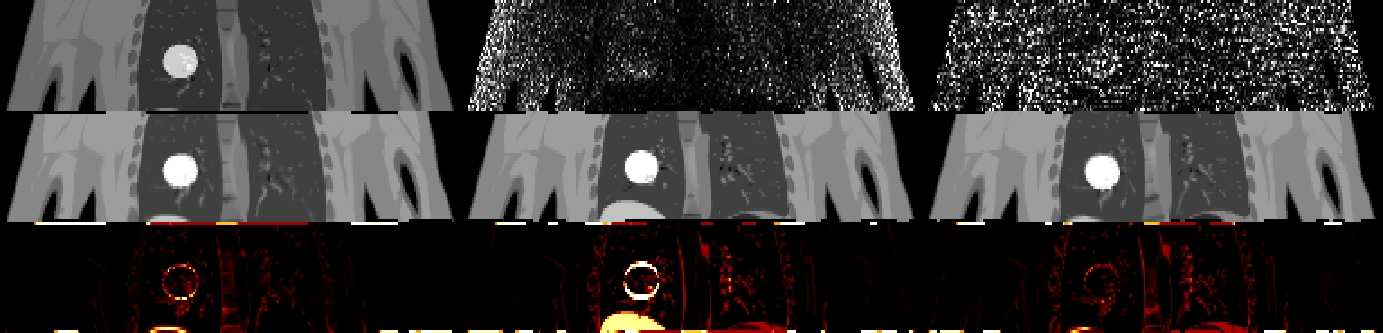
\includegraphics[width=1\linewidth]{output_flipped.png}
    \caption{All volumes correspond to end-inhalation. First row from left to right: XCAT PET data, NAC nonTOF reconstructed data and NAC TOF reconstructed data. Second row: RCM applied to mean position XCAT data with RCM derived from XCAT PET data (left), NAC nonTOF (middle) and NAC TOF (right) volumes. Colour map ranges are consistent for all images on this row. The third row from left to right: The difference between the estimated volumes from the second row with the XCAT end-inhalation volume. Colour map ranges are consistent for all images on this row.}
    \label{fig:output}
\end{figure*}

\begin{multicols}{2}

\begin{table}[H]
    \centering
    \caption{Comparison of the MSE between the ground truth data and the volumes estimated from the RCMs.}
    
    \vspace{1.0cm}
    
    \scalebox{1.6}
    {
        \begin{tabular}{||c|ccc||}
            \hline
                \textbf{MSE}    & \textbf{XCAT} & \textbf{nonTOF}   & \textbf{TOF}  \\
            \hline
                \textbf{$1$}    & $24707$       & $20020$           & $31370$       \\
                \textbf{$2$}    & $28595$       & $39309$           & $30445$       \\
                \textbf{$3$}    & $24242$       & $75570$           & $35417$       \\
                \textbf{$4$}    & $26127$       & $59310$           & $32519$       \\
                \textbf{$5$}    & $26459$       & $12951$           & $26120$       \\
                \textbf{$6$}    & $24707$       & $20020$           & $31370$       \\
            \hline
                \textbf{Mean}   & $26026$       & $41432$           & $31174$       \\
            \hline
        \end{tabular}
    }
    \label{tab:mse}
\end{table}

\begin{figure}[H]
    \centering
    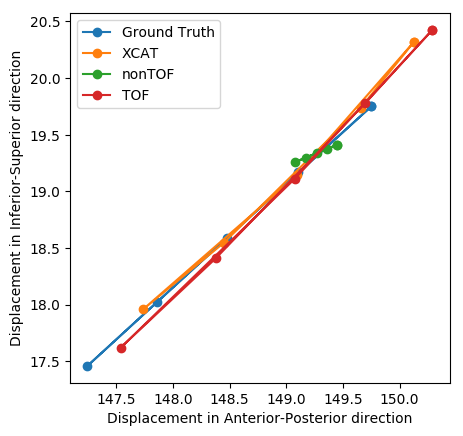
\includegraphics[width=0.6\linewidth]{com_graph.png}
    \caption{The path of the COM of the lesion.}
    \label{fig:com_graph}
\end{figure}

\end{multicols}
\begin{multicols}{4}
\large

\section*{Results}
We compared $3$ RCMs, calculated from the PET XCAT volumes, nonTOF NAC reconstructions and TOF NAC reconstructions. The $3$ RCMs were used to warp the PET volume generated by XCAT at the mean breathing position to position at each gate. These estimated volumes were then compared to the original XCAT input volumes. First, differences volumes were obtained by subtracting the original XCAT volume and warped volumes at the same gate. \textcolor{UCLburgundy}{\textbf{The mean MSE was found to be lower for the NAC TOF data than for the NAC nonTOF.}} In addition, the centre of mass (COM) of the lesion was also tracked, by warping a volume only including the lesion in the reference position. \textcolor{UCLburgundy}{\textbf{The path of the NAC TOF data follows the ground truth path much closer than the NAC nonTOF data.}}

\section*{Conclusions}
\textcolor{UCLburgundy}{\textbf{Motion models derived from NAC TOF volumes were found to be more robust than when using NAC nonTOF, both visually and when comparing MSE and COM.}} This is likely due to the improved image contrast of NAC TOF images. In the future, research will focus on investigating the robustness of the motion model estimation to different noise levels, acquisition duration and size of lesion.

\AtNextBibliography{\small}
\printbibliography

\small
\section*{Acknowledgements}
This research is supported by GE Healthcare, the NIHR UCLH Biomedical Research Centre and the EPSRC-funded UCL Centre for Doctoral Training in Medical Imaging (EP/L016478/1).
Elise~C.~Emond is supported by GlaxoSmithKline (BIDS3000030921).

\end{multicols}
\end{document}
